%##########################  CHAPER 6: APPLICATION  #######################

\chapter{Entwicklung der Anwendung}\label{kap:application}


Dieses Kapitel beschreibt die Entwicklung der Anwendung,
welche als autonomes System dass auf einem Raspberry Pi 4 läuft.

Dazu gehören die Einrichtung einer infrarotfähigen 
Kamera, die Implementierung der Inferenz mit OpeVino
und die Verbindung zu einem Pc zur übertragung
der Daten mit geeignetem Protokolls.



%-------------------------  SECTION 1: AUFBAU  ------------------------
\section{Aufbau/Hardware}\label{sec:aufbau}


Der Aufbau besteht aus einem Raspberry Pi, auf welche 
der Anwendungscode läufr, dem NCS2 für die Inferenz, 
welcher per USB mit dem Raspberry verbunden wird.

Desweiteren wurde ein Raspberry Pi Kamera Modul mit 
5MP OV5647 Sensor der Marke Longrunner verwendet.

Dieses ermöglicht durch zu und abschalten eines Infrarot 
Filters vor die Linse zwischen Tag und Nachtsicht zu wechseln.

Das Schalten wird dabei über einen Helligkeitssensor automatisch 
geregelt. Im Infrarotmodus bfindet sich der Infrarot Filter nicht 
vor der linse, wodurch auch die etwas längeren (850nm)
Elektromagnetischen Wellen als die des Sichtbaren Lichts aufgenommen 
werden können.

Durch zwei Infrarot LEDs des gleichen Spektrums, können so 
auch in der Dunkelheit Bilder aufgenommen werden, ohne 
Sichtbare beläuchtung, was Tiere verscheuchen würde.


Das kamera Modul wird über die CSI (Camera Serial Interface) 
Schnittstelle mit dem Raspberry Pi verbunden.


%https://www.amazon.de/gp/product/B07R4JH2ZV/ref=ppx_yo_dt_b_asin_title_o01_s00?ie=UTF8&psc=1


\begin{minipage}{0.55\textwidth}
    \centering
    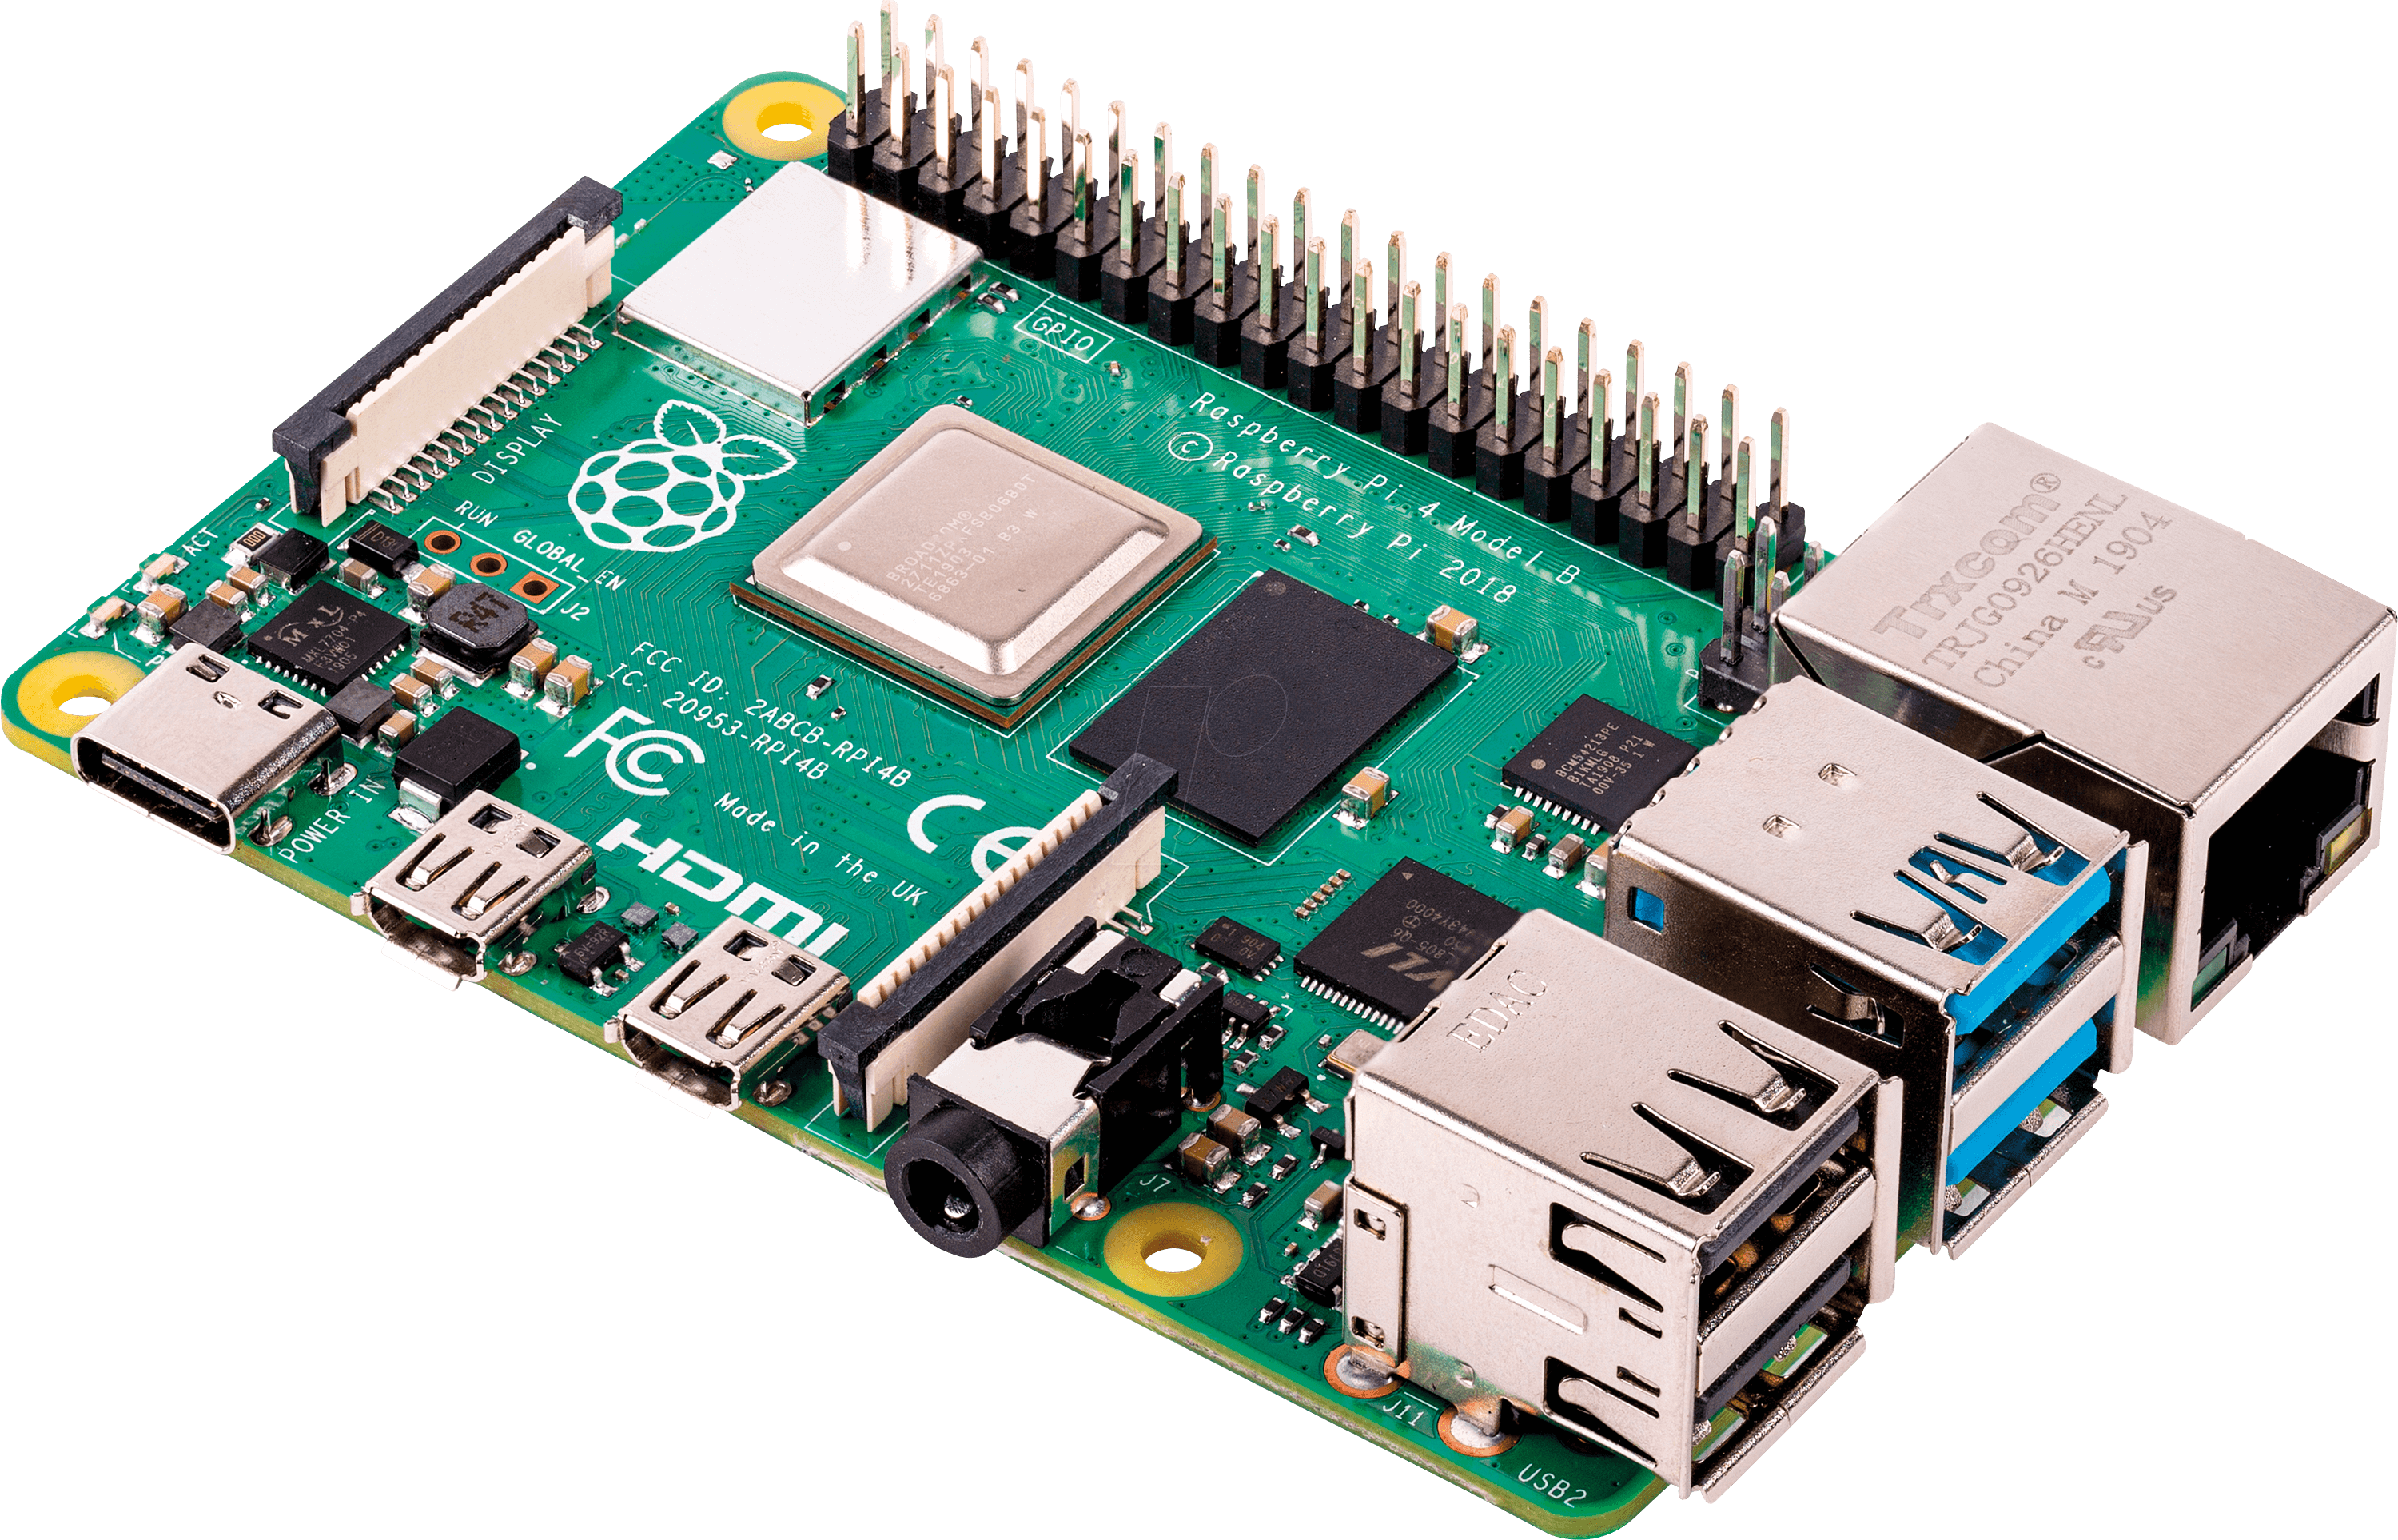
\includegraphics[width=0.8\textwidth]{./Bilder/raspberrypi_4.png}
    \captionof{figure}{Raspberry Pi 4}
    \label{img:raspberrypi}
\end{minipage}
\begin{minipage}{0.45\textwidth}
    \centering
    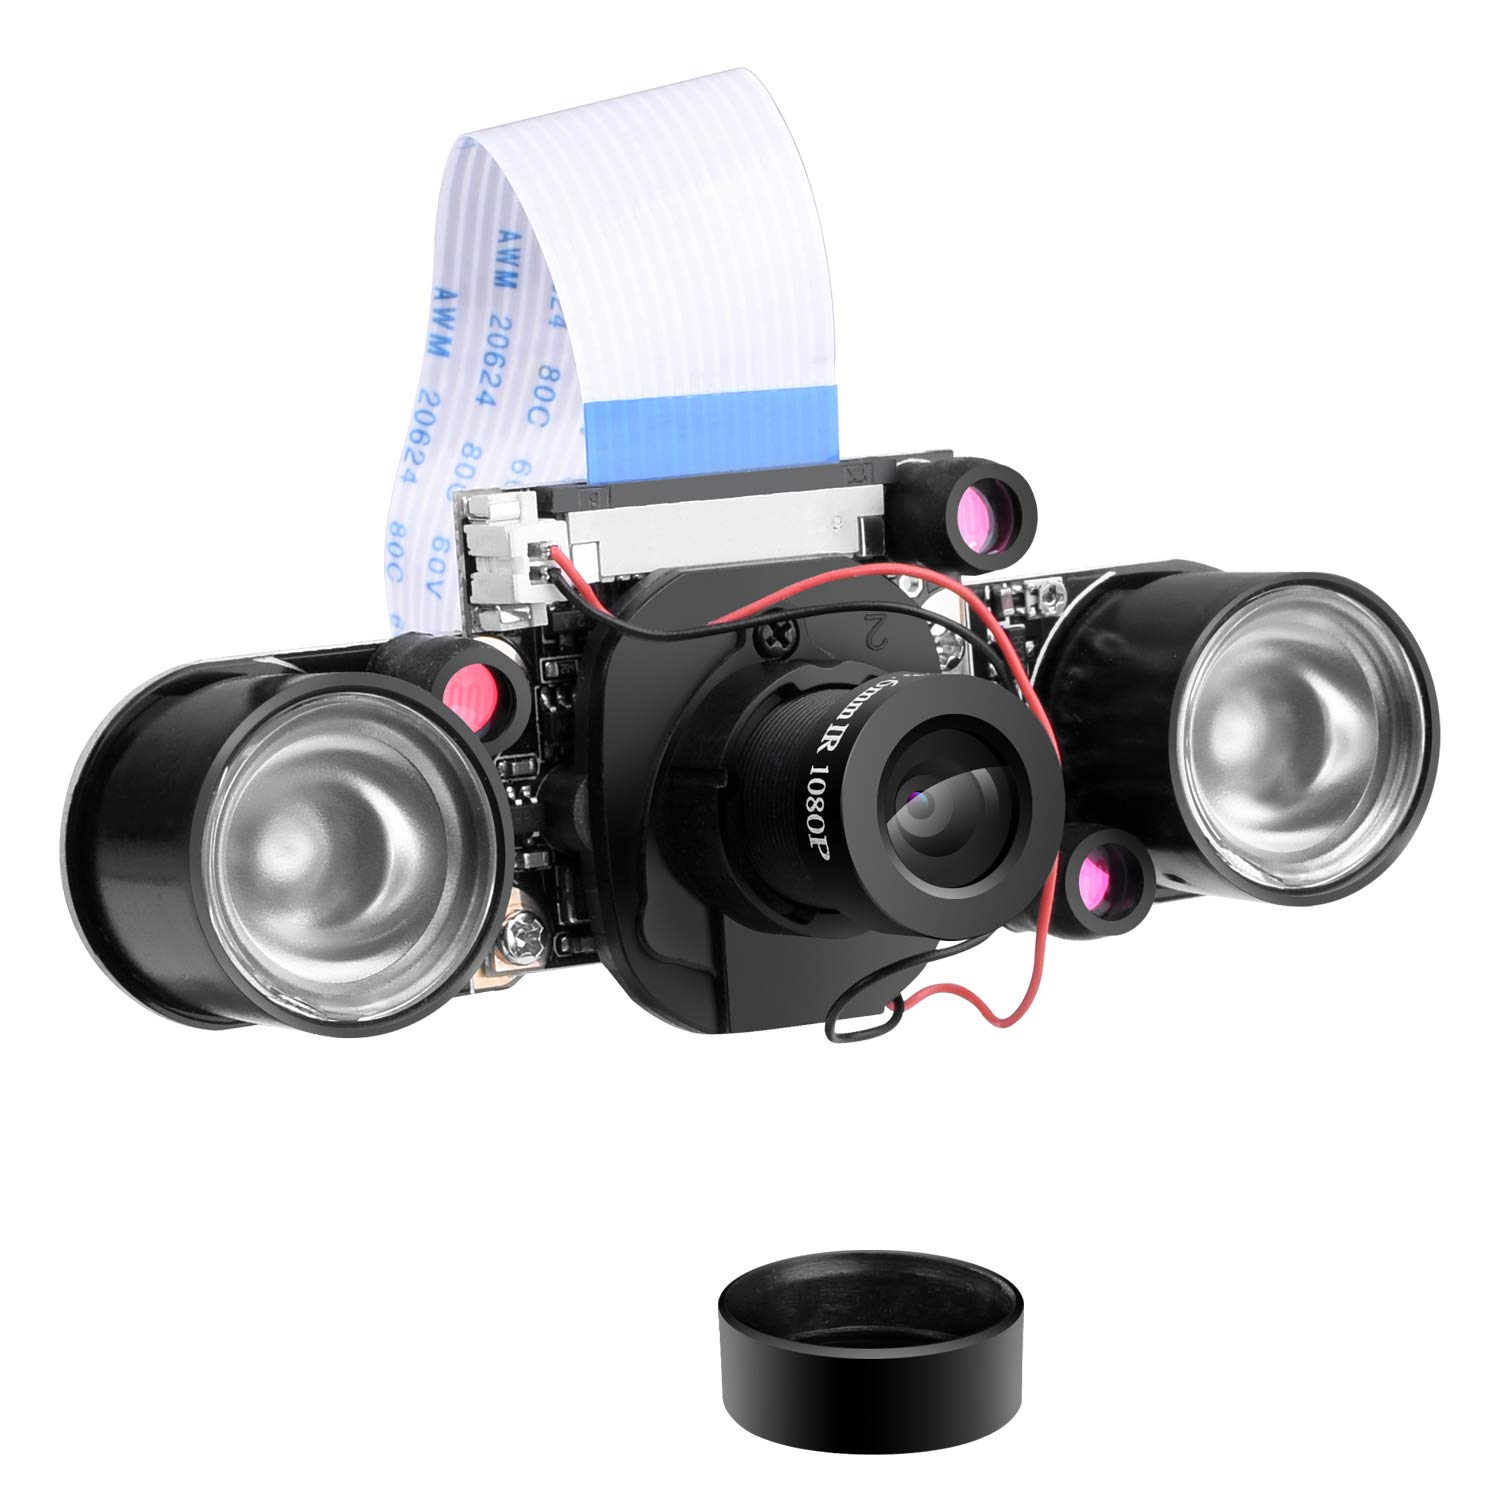
\includegraphics[width=0.8\textwidth]{longrunner.jpg}
    \captionof{figure}{Longruner Kamera Modul}
    \label{fig:rpicam}
\end{minipage}
\vspace{0.6cm}


Desweiteren wurde für eine mobile Internetverbindung 
der \textit{Huawei E3531 SurfStick} und zu Stromversorgnung
eine Powerbank verwendet.


% https://www.amazon.de/gp/product/B00HSZEY34/ref=ppx_yo_dt_b_asin_title_o00_s00?ie=UTF8&psc=1


\section{Implementierung/Software}

Die Implementierung der Anwendung wurde in Python vorgenommen und 
besteht aus den drei Scripten \texttt{main.py}, \texttt{detection.py}
und \texttt{connection.py}. Welche Folgend dargestellte Klassen 
implementieren.

\vspace{1cm}
\begin{tikzpicture} 

    
    
            \umlclass{Motion}{ 
              statickBackground : np.array
              }{ 
              + detectMotion() : bool \\
              + resetBackground() : void
            }
        
            \umlclass[y=-4]{InferenceModel}{ 
                string : plugin
                strin : device
                }{ 
                + createExecInferModel() : ExecInferModel
              }
        
            \umlclass[y=-2, x=6]{ExecInferModel}{ 
                shape : ioBlob\\
                detected : array
                }{ 
                + inferFrames() : status \\
                \# status[0] num infered\\
                \# status[1] num detected\\
                \# status[2] num saved\\
                - save() : void
                }
        
    
        \umlclass[x=11, y=-2]{Connection}{ 
            string logindata
            }{ 
            + login() : bool \\
            + connect() : server, port\\
            + send() : bool\\
            + disconnect() : bool\\
            + sendEmail(email, text) : boiol
          }

    
    \end{tikzpicture}
        
\vspace{1cm}

Dabei führt die Main Anwendung eine Dauerschleife aus, in der 
die Frames der Kamera erhalten werden. 

Die inferenz wird über das detection Script, welches die 
InferenceEngine implementier ausgeführt.
Das senden erkannter Ergebnisse erfolgt dann mithilfe 
des Detection Scripts.


Um trotz der langsamen Inferenz Zeit das Faster R-CNN 
verwenden zu können, galt es die Anwendung und die 
Zeitliche ausführungen der Inferenz so zu gestallten, 
das möglichst alle Frames, in welchen Tiere zu beobachten 
sein können, auch inferiert werden.

Dafür wurde die Annahme gemacht, dass zur Laufzeit der 
Anwendung häufig Zeiten sind in denen nichts zu inferieren 
ist, was durch eine Bewegungserkennung herausgefunden werden 
konnte.

Desweiteren wurde die Inferenz so implementiert, dass sie 
im gegensatz zur üblichen verwendung an keiner stelle Blockiert, 
wodurch durch zwischen Speichern von Bildern in denen 
Bewegung erkannt wurde trotz langsamerer Inferenzzeit alle 
Frames inferiert werden können.

Folgendes Diagramm zeigt schmematsch den groben Ablauf davon.

\vspace{1cm}


\begin{center}
\tikzset{
    desicion/.style={
        diamond,
        draw,
        text width=4em,
        text badly centered,
        inner sep=0pt
    },
    block/.style={
        rectangle,
        draw,
        text width=10em,
        text centered,
        rounded corners
    },
    arrow/.style={
        draw,
        >=latex,
        ->
    }
}


\begin{tikzpicture}
    \node (A) [desicion] {entschei\\dung};
    \node (B) [block, below of=A, node distance=3cm, text width=5em] {bock};
    \node (C) [block, right of=A, node distance=0.5\textwidth] {noch ein\\bock};


    \draw[arrow] (A) --  node [left, fill=white!30] {yes} (B);
    \draw[arrow] (A) -- node [below, near end] {crap} (C); 
    \draw[arrow] (B) -| node [near start, fill=white] {yes} (C);

\end{tikzpicture}

\end{center}

\subsection{Inferenz}

\subsubsection{Motion}

Die Bewegungserkennung wurde mithilfe der Library OpenCV implementiert, indem
zu beginn ein Frame als Refernz abgespeichert wurde.
Mit diesem konnten dann alle weiteren Input frames vergleichen werden 
indem der Abstand der einzelnen Pixel werte berechnet und gemittelt wird.
Beträgt dieser mehr als ein bestimmter threshhold wird das als Bewegung 
gewertet.

\subsubsection{Inferenz}

Die in Abschnitt \ref{sec:infertime} beschriebene asynchrone 
Inferenz wurde dahingehend abgeändert, dass nun theoretsch belibieg file 
Requests verwendete werden können und für den wait Befehl der 
Timeout auf 0ms gesetzt wurde und so der Ablauf nicht mehr Blockierend 
ist. Dadurch kann die Inferenz unabhängig von der Frequenz der 
von der Kamera erhaltenen Bilder ablaufen.
Auf eine richtige zuordnung der Inferenz ergebnisse zu dem 
jeweiligen verwendeten Frame war zu achten.


\begin{algorithm}[H]
    \caption{Asynchrone Inferenz, ohne Blockierung}
    \begin{algorithmic}
    \WHILE{\TRUE}
    \STATE capture FRAMES
        \FOR{ReqNr in all InferRequests}
            \STATE status \textbf{wait} for ReqNr
            \IF {status == 0}
                \STATE res = ReqNr.output
            \ENDIF
            
            \IF {Buffer != 0}
                \STATE preprocess ReqNr
                \STATE \textbf{statr} ReqNr
            \ENDIF

            \IF{res != NULL}
                \STATE process result
            \ENDIF
        \ENDFOR
    \ENDWHILE
    \end{algorithmic}
\end{algorithm}    



\subsection{Conncection/Verbindung}


Um eine Verbindung zwischen Raspberry Pi und Pc herzustellen, 
die unabhängig davon ob sich die geräte im selben 
Netzwerk befinden funktioniert, wurde eine Cloud Proxy Verbindung 
implementerit.

Dafür wurde der Dienst \textit{remot3.it} \cite{remoteit} verwendet, 
mit dem es möglich ist ohne Konfiguration des Routers eine
Netzwerkübergreifende Remote Verbindung zum Raspberry Pi herzustellen.

Da die Daten vom Raspberry aus automatisch gesendet werden sollen, 
wurde der Pc als Remote Gerät implementerit un auf dem Raspberry 
eine SSH Verbindung zum Pc hergestellt.


\begin{figure}[H]
    \centering
    \def\svgwidth{0.7\textwidth}
    \input{Bilder/diagram-connect.pdf_tex}
    \caption{}
    \label{}
\end{figure}


Dafür bot remot3.it eine API die es ermöglicht über Get und Post Requests
den Verbindung auf und Abbau zu automatisieren.

Gesendet wurden die Daten dann per SCP Command (Secure Copy Protocol), 
welches die aufgaebaute SSH Verbiindung verwendet.













% \input{Bilder/class_diagramm/class_diagramm.latex}

% \begin{minipage}{0.3\textwidth}
%     \centering
%     \input{Bilder/diagramme/class_detection.tex}    
% \end{minipage}
% \begin{minipage}{0.3\textwidth}
%     \centering
%     \input{Bilder/diagramme/class_connection.tex}
% \end{minipage}
% \begin{minipage}{0.3\textwidth}
%     \centering
%     \input{Bilder/diagramme/class_motion.tex}
% \end{minipage}

% oder

%\input{Bilder/diagramme/detection_package.tex}

% oder 





%Asynchrone inferenz
%https://docs.openvinotoolkit.org/latest/_demos_python_demos_object_detection_demo_ssd_async_README.html

% main
% \begin{algorithm}[H]
%     \caption{Main Program}
%     \begin{algorithmic}

%     %\STATE INIT EXEC_NET, CAM

%     \WHILE{\TRUE}
%         \STATE capture frame
        
%         \IF{frame has motion}
%             \STATE $buffer \leftarrow frmae$
%         \ENDIF

%         \IF{buffer is empty}
%             \STATE disconnect
%         \ENDIF

%         \STATE result = inferFrames (buffer)

%         \FOR{all results}
%             \STATE process results
%             \IF {saved}
%                 \STATE sendRequest = \TRUE
%             \ENDIF
        

%             \IF {no detectoin for 20 times}
%                 \STATE reset motion background
%                 \STATE delete buffer
%                 \IF {connected}
%                     \STATE disconnect
%                 \ENDIF
%             \ENDIF

%         \ENDFOR

%         \IF {send all every minute}
%             \STATE save current detections
%             \STATE sendRequest = \TRUE
%         \ENDIF

%         \IF{sendRequest == \TRUE}
%             \IF{not logged in}
%                 \STATE log in
%             \ENDIF

%             \IF{not connected}
%                 \STATE connect
%             \ENDIF

%             \STATE server, port $\leftarrow$ connection

%             \STATE sendRequest = \FALSE
%             \FOR{all saved images}
%                 \IF{send image $\rightarrow$ server, port}
%                     \STATE delete image
%                 \ELSE
%                     \STATE sendRequest = \TRUE
%                 \ENDIF
%             \ENDFOR

%         \ENDIF
%     \ENDWHILE


%     \end{algorithmic}
% \end{algorithm}



% \newpage

% \begin{center}
%     \rule{0.8\textwidth}{0.4pt}
%     \begin{lstlisting}[language=Python]
%         def infer_frames(Buffer, threshhold):
%             for idx, inferRequest in all inferRequests:
%                 status = inferRequest.wait(0) # nicht blockierend
%                 if status not ready:
%                     continue
                
%                 if idx in currentFrames:
%                     results = inferRequest.output
%                     frame = currentFrames[idx]

%                 if Buffer not empty:
%                     currentFrames[idx] = Buffer.pop()
%                     infer_frame = preprocess(currentFrames[idx])
%                     inferRequest.async_infer(infer_frame)

%                 if results or frame is None:
%                     continue

%                 for obj in all results:
%                     Class, Roi, Proba <- obj
%                     if Proba < threshhold:
%                         continue
                    
%                     coords <- Roi, frame.shape

%                     infered_frame = draw_rect(frame, coords)

%                     if proba > detectedObjects.proba
%                         replace detectedObjects

%                     if number of detections > x:
%                         send(frame)
                    
%     \end{lstlisting}
%     \rule{0.8\textwidth}{0.4pt}        
% \end{center}


% \centering\rule{0.6\textwidth}{0.4pt}
% \begin\centering{lstlisting}[language=Python]
%     def infer_frames():
%         for all requests:
%             do something \textbf{with} request

%             status = request.wait(0)
%             if status == done:
%                 res = requests.output
%                 frame = current[id]
% \end{lstlisting}
% \centering\rule{0.6\textwidth}{0.4pt}




% % inferenz
% \begin{algorithm}[H]
%     \caption{Asynchrone Inferenz}
%     \begin{algorithmic}
%     \WHILE{\TRUE}
%         \STATE capture Frame
%         \IF{Frame has Motion}
%             \STATE Buffer $\leftarrow$ Frame
%         \ENDIF
%         \FOR{$reqId$ = 0 to $reqMax$}
%             \IF {Model.reqests[$reqId$].wait(0)}
%                 \STATE result = Model.reqests[$reqId$].output
%                 \STATE inferedFrames $\leftarrow$ (result, currentFrames[$reqId$])
%                 \IF {Buffer not empty}
%                     \STATE currentFrames[$reqId$] $\leftarrow$ Buffer 
%                     \STATE inFrame = preprocess: currentFrames[$reqId$]
%                     \STATE Model.inferAsync($reqId$, inFrame)
%                 \ENDIF
%             \ENDIF
%         \ENDFOR
%         \RETURN inferedFrames
%     \ENDWHILE
%     \end{algorithmic}
% \end{algorithm}

% wobei die wait Funktion mit Timeout = 0 nicht blockierend ist.

% Dadurch war es möglich trotz langsamerer inferenz zeit als 
% capture zeit, durch zwischenspeichern alle frames zu inferieren, 
% unter der Annahme, das nur zeitweise bewegung erkannt und damit 
% inferiert werden muss.



